By making an analogy with the Non-Commutative Stone Duality of Lawson-Lenz, between certain classes of groupoids and inverse semigroups, we look at the following question: How can one recover an inverse semigroupoid from its set of bisections?

Let $\mathcal{S}$ be a discrete inverse semigroupoid. Then the set $\mathbf{B}(\mathcal{S})$ of bisections of $\mathcal{S}$ is an inverse semigroup under product of sets. However, the natural order in this semigroup does not coincide with set inclusion: Given $A,B\in\mathbf{B}(\mathcal{S})$, we have $A\leq B$ if and only if for all $a\in A$, there exists $b\in B$ with $(\ra(b),\so(b))=(\ra(a),\so(a))$ and $a\leq b$.

As a more concrete example, if $S$ is an inverse semigroup, then the non-empty bisections of $S$ are simply singleton sets, and thus set inclusion coincides with identity: $\left\{a\right\}\subseteq\left\{b\right\}$ if and only if $a=b$. However, as long as $S$ is not a group, there will be distinct elements $a\neq b$ with $a\leq b$.

Therefore, in order to recover $\mathcal{S}$ from $\mathbf{B}(\mathcal{S})$ we will need to consider information about set containment as well.

Following the approach in classical Stone duality, as well as in the initial versions of non-commutative Stone duality for groupoids, we will consider only locally compact étale semigroupoids with Hausdorff and zero-dimensional idempotent spaces.

\begin{lemma}\label{lem:ES.Hausdorff.and.S0.Hausdorff}
    Suppose that $\mathcal{S}$ is a topological inverse semigroupoid.
    \begin{enumerate}[label=(\alph*)]
        \item\label{lem:ES.Hausdorff.and.S0.Hausdorff1} If $E(\mathcal{S})$ is Hausdorff and , then $\mathcal{S}^{(0)}$ is Hausdorff as well.
        \item\label{lem:ES.Hausdorff.and.S0.Hausdorff2} If $\mathcal{S}^{(0)}$ is Hausdorff, then the product of compact subsets of $\mathcal{S}$ is compact.
    \end{enumerate}
\end{lemma}
\begin{proof}
    \begin{enumerate}[label=(\alph*)]
    \item Suppose $E(\mathcal{S})$ is Hausdorff. Given $x_1\neq x_2$ in $\mathcal{S}^{(0)}$, choose $e_1,e_2\in E(\mathcal{S})$ with $\so(e_i)=x_i$, so $e_1\neq e_2$. Take any two open bisections $U_1,U_2$ with $e_i\in U_i$. 
    \item We have $\mathcal{S}^{(2)}=\left\{(a,b)\in\mathcal{S}\colon \so(a)=\ra(b)\right\}$, which is closed in $\mathcal{S}\times\mathcal{S}$ as $\so$ and $\ra$ are continuous and $\mathcal{S}^{(0)}$ is Hausdorff.
    
    If $\mu\colon\mathcal{S}^{(2)}\to\mathcal{S}$ denotes the (continuous) product, then for any two compact subsets $K,L\subseteq\mathcal{S}$, $(K\times L)\cap\mathcal{S}^{(2)}$ is closed in the compact $K\times L$, hence compact itself. Therefore $KL=\mu((K\times L)\cap\mathcal{S}^{(2)})$ is compact.\qedhere
    \end{enumerate}
\end{proof}


\begin{example}
Let $X$ be any Hausdorfff topological space with a non-isolated point $x_0$., and let $L_2=\left\{0,1\right\}$ be the lattice with $0\leq 1$. Let $\mathcal{S}$ be the inverse semigroupoid obtained from $L_2\times X$ by identifying $(0,x)$ with $(1,x)$ whenever $x\neq x_0$. Then $\mathcal{S}=E(\mathcal{S})$ is a non-Hausdorff, étale inverse semigroupoid, and $\mathcal{S}^{(0)}=X$ is Hausdorff.

Now consider $Y=\mathcal{S}$ simply as a topological space. Let $E=\left\{0,a,b\right\}$ be the semilattice with $x\leq y\iff x=0\text{ or }x=y$, and $\mathcal{T}=E\times X\setminus\left\{(0,x_0)\right\}$, which we make an inverse semigroupoid over $Y$ as follows: If $\so(a,x_0)$ is the class of $(0,x_0)$ in $Y$, $\so(b,x_0)$ is the class of $(1,x_0)$ in $Y$, and if $x\neq x_0$, then $\so(e,x)$ is the class of $(0,x)$ in $Y$. Then the product of $E\times X$ restricted to $\mathcal{T}$ makes it a Hausdorff, étale inverse semigroupoid, with non-Hausdorff vertex space.

\[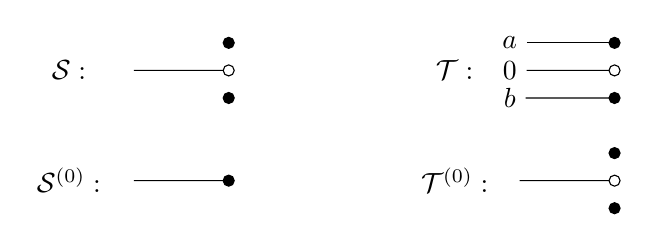
\begin{tikzpicture}[scale=0.7]
\node (SS0) at (0,0) {};
\draw[fill=black] ([shift={+(-0.1,0)}]SS0) circle (0.1);
\node (start_X) at ([shift={+(-2,-0.5)}]SS0) {};
\node (end_X) at ([shift={+(2,0)}]start_X) {};
\draw[-] (start_X)--(end_X);
\draw[fill=white] ([shift={+(-0.1,0)}]end_X) circle (0.1);
\node (Y1) at ([shift={+(0,-0.5)}]end_X) {};
\draw[fill=black] ([shift={+(-0.1,0)}]Y1) circle (0.1);
\node (start_S0) at ([shift={+(0,-2)}]start_X) {};
\node (end_S0) at ([shift={+(2,0)}]start_S0) {};
\draw[-] (start_S0)--(end_S0);
\draw[fill=black] ([shift={+(-0.1,0)}]end_S0) circle (0.1);

\node (S) at ([shift={+(-1,0)}]start_X) {$\mathcal{S}:$} ;
\node (S0) at ([shift={+(-1,0)}]start_S0) {$\mathcal{S}^{(0)}:$} ;

\node (start_a) at ([shift={+(5,0)}]SS0) {$a$};
\node (end_a) at ([shift={+(2,0)}]start_a)  {};
\draw[-] (start_a)--(end_a);
\draw[fill=black] ([shift={+(-0.1,0)}]end_a) circle (0.1);
\node (start_0) at ([shift={+(0,-0.5)}]start_a) {$0$} ;
\node (end_0) at ([shift={+(2,0)}]start_0)  {};
\draw[-] (start_0)--(end_0) ;
\draw[fill=white] ([shift={+(-0.1,0)}]end_0) circle (0.1);
\node (start_b) at ([shift={+(0,-0.5)}]start_0) {$b$} ;
\node (end_b) at ([shift={+(2,0)}]start_b)  {};
\draw[-] (start_b)--(end_b) ;
\draw[fill=black] ([shift={+(-0.1,0)}]end_b) circle (0.1);
\node (Y0) at ([shift={+(0,-1)}]end_b) {};
\draw[fill=black] ([shift={+(-0.1,0)}]Y0) circle (0.1);
\node (start_X) at ([shift={+(-2,-0.5)}]Y0) {};
\node (end_X) at ([shift={+(2,0)}]start_X) {};
\draw[-] (start_X)--(end_X);
\draw[fill=white] ([shift={+(-0.1,0)}]end_X) circle (0.1);
\node (Y1) at ([shift={+(0,-0.5)}]end_X) {};
\draw[fill=black] ([shift={+(-0.1,0)}]Y1) circle (0.1);

\node (T) at ([shift={+(-1,0)}]start_0) {$\mathcal{T}:$} ;
\node (T0) at ([shift={+(-1,0)}]start_X) {$\mathcal{T}^{(0)}:$} ;
\end{tikzpicture}
\]
\end{example}
\begin{definition}
    An étale inverse semigroupoid $\mathcal{S}$ is \emph{ample} if $\mathcal{S}^{(0)}$ is locally compact, Hausdorff and zero-dimensional. We denote by $\mathbf{KB}(\mathcal{S})$ the inverse semigroup of compact-open bisections of $\mathcal{S}$.
\end{definition}

We now axiomatize set inclusion for $\mathbf{KB}(\mathcal{S})$. For a preorder $\subseteq$ on an inverse semigroup $S$, we denote respective joins and meets by $a\cup b=\sup_{\subseteq}\left\{a,b\right\}$ and $a\cap b=\inf_{\subseteq}\left\{a,b\right\}$, whenever either exists.

\begin{definition}\label{def:sigmaorder}
A \emph{$\Sigma$-ordered} inverse semigroup is an inverse semigroup with zero $S$ equipped with a compatible order $\subseteq$ satisfying
\begin{enumerate}[label=($\Sigma$-\roman*)]
    \item\label{def:sigmaorder.0minimum} $0\subseteq a$ for all $a\in S$.
    \item\label{def:sigmaorder.conditionaljoins} $(S,\subseteq)$ admits \emph{conditional joins}: If $a_1,a_2\subseteq c$, then the join $a_1\cup a_2=\sup_{\subseteq}\left\{a_1,a_2\right\}$ exists.
    \item\label{def:sigmaorder.distributivity} $(S,\subseteq)$ is (finitely) \emph{distributive}: If a join $c_1\cup c_2$ exists and $a\in S$, then $a(c_1\cup c_2)=(ac_1)\cup (ac_2)$ (the latter term exists by the previous item).
    \item\label{def:sigmaorder.ESrelativecomplements} $(E(S),\subseteq)$ admits relative complements: If $e\subseteq f$ in $E(S)$, then there exists a $c\in E(S)$ such that $e\cup c=f$ and $e\cap c=0$. Such $c$ is necessarily unique (see next paragraph), and denoted by $f\setminus e$.
    \item\label{def:sigmaorder.zerojoins} If $a^*b=ab^*=0$, then the join $a\cup b$ exists.
    \item\label{def:sigmaorder.interpolation} If $t\leq a$ in $S$, then there exists $z\subseteq a$ such that $t\leq z\subseteq a$ and
    \[tx=0\iff zx=0\qquad\text{ for all }x\in S.\]
\end{enumerate}
\end{definition}

The proof that relative complements of $(E(S),\subseteq)$ are unique follows as in the classical setting by distributivity: If $e\subseteq f$ in $E(S)$ and $c_1,c_2$ are relative complements of $e$ in $f$, then $c_1e=c_1\cap e=0$ (see Lemma \ref{lem:technicalpropertiesofsigmaorder}\ref{lem:technicalpropertiesofsigmaorder3}), so
\[c_1=c_1f=c_1(e\cup c_2)=c_1e\cup c_1c_2=0\cup c_1c_2=c_1c_2\]
i.e., $c_1\leq c_2$, and symmetrically we conclude that $c_1=c_2$.

Since compatible orders are preserved by taking inverses, then property \ref{def:sigmaorder.distributivity} implies $(c_1\cup c_2)a=(c_1a)\cup(c_2a)$ as well.

In the next few technical lemmas, we compile the technical properties of $\Sigma$-ordered inverse semigroups which will be necessary, and follow the discussion with two canonical examples. Let us fix, throughout this subsection, a $\Sigma$-ordered inverse semigroup $(S,\subseteq)$.

\begin{lemma}\label{lem:technicalpropertiesofsigmaorder}
Suppose that $(S,\subseteq)$ is a $\Sigma$-ordered inverse semigroup.
    \begin{enumerate}[label=(\alph*)]
        \item\label{lem:technicalpropertiesofsigmaorder1} If $x\leq y\leq z$ and $x\subseteq z$, then $x\subseteq y$.
        \item\label{lem:technicalpropertiesofsigmaorder2} If $a\cap b$ exists and $c\subseteq b$, then $a\cap c$ exists, and $a\cap c=(a\cap b)c^*c$.
        \item\label{lem:technicalpropertiesofsigmaorder3} If $x,y\subseteq a$, then $x\cap y$ exists, and $x\cap y=xy^*y=yy^*x$.
        \item\label{lem:technicalpropertiesofsigmaorder4} If $x,y\subseteq a$ and $b\in S$, then $b(x\cap y)=bx\cap by$.
        \item\label{lem:technicalpropertiesofsigmaorder5} If $a\cup b$ exists, then $(a\cup b)^*(a\cup b)=a^*a\cup b^*b$
        \item\label{lem:technicalpropertiesofsigmaorder6} If $b\cup c$ exists, then
        \[a\cap(b\cup c)=(a\cap b)\cup(a\cap c)\]
        in the sense that one side is defined if and only if the other one is, in which case they coincide.
        \item\label{lem:technicalpropertiesofsigmaorder7} $S$ admits relative complements. More precisely, if $a\subseteq b$, then $b\setminus a=b(b^*b\setminus a^*a)$. (Note that the relative complement $b^*b\setminus a^*a$ is defined by \ref{def:sigmaorder.ESrelativecomplements}.)
        \item\label{lem:technicalpropertiesofsigmaorder8} If $a\cup b$, $a\cup c$ and $b\cap c$ are defined, then
        \[a\cup(b\cap c)=(a\cup b)\cap (a\cup c)\]
        in the sense that both sides are defined and coincide.
        \item\label{lem:technicalpropertiesofsigmaorder9} If $a\subseteq b$ and $c\in S$, then $c(b\setminus a)=(cb)\setminus (ca)$.
        \item\label{lem:technicalpropertiesofsigmaorder10} (De Morgan's Laws) If $a_1,a_2\subseteq b$ then $(b\setminus a_1)\cap(b\setminus a_2)=b\setminus(a_1\cup a_2)$ and $(b\setminus a_1)\cup(b\setminus a_2)=(b\setminus a_1\cap a_2)$.
    \end{enumerate}
\end{lemma}
\begin{proof}
    \begin{enumerate}[label=(\alph*)]
        \item As $x\subseteq z$, we multiply both sides by $y^*y$ to obtain $x=xy^*y\subseteq zy^*y=y$, because $x\leq y\leq z$.
        \item On one hand, $(a\cap b)c^*c\subseteq (a\cap b)b^*b=a\cap b\subseteq a$, and $(a\cap b)c^*c\subseteq bc^*c=c$, so $(a\cap b)c^*c$ is a $\subseteq$-lower bound of $\left\{a,c\right\}$. Simple computations prove that it is the greatest lower bound.
        \item This was already proven in Lemma \ref{lem:relation.of.germs.is.a.graphed.congruence}.
        \item As $bx,by\subseteq ba$, item \ref{lem:technicalpropertiesofsigmaorder2} yields $bx\cap by=bx(by)^*(by)$. As $x,y\leq a$, then $xy^*\in E(S)$, so we may commute $xy^*$ and $b^*b$ to obtain
        \[bx\cap by=b(xy^*)(b^*b)y=b(b^*b)(xy^*)y=b(x\cap y)\]
        where we used item \ref{lem:technicalpropertiesofsigmaorder2} in the last equality, as $x\cap y=xy^*y$.
        
        \item By distributivity, Property \ref{def:sigmaorder.distributivity},
        \[(a\cup b)^*(a\cup b)=(a^*\cup b^*)(a\cup b)=(a^*a)\cup(a^*b)\cup(b^*a)\cup(b^*b).\]
        But since $a^*b\subseteq a^*(a\cup b)=a^*a$, and similarly for $b^*a$, then
        \[(a\cup b)^*(a\cup b)=a^*a\cup b^*b.\]
        
        \item If $a\cap(b\cup c)$ exists, then item \ref{lem:technicalpropertiesofsigmaorder5} implies that both $a\cap b$ and $a\cap c$ exist, Since both are $\subseteq a$, their $\subseteq$-join exists by Property \ref{def:sigmaorder.conditionaljoins}.
        
        Assume now that $(a\cap b)\cup(a\cap c)$ exists, and let us prove that it is the $\subseteq$-meet of $\left\{a,b\cup c\right\}$. It is a lower bound, since
        \[(a\cap b)\cup(a\cap c)\subseteq a\cup a=a\quad\text{and}\quad (a\cap b)\cup(a\cap c)\subseteq b\cup c.\]
        To prove that it is the largest lower bound, suppose $p\subseteq a$ and $p\subseteq (b\cap c)$. In particular, $p\cap b=b$. As $a\cap b$ exists, item \ref{lem:technicalpropertiesofsigmaorder5} implies $(a\cap b)p^*p=p\cap b=p$. Similarly, $(a\cap c)p^*p=p$. By distributivity, Property \ref{def:sigmaorder.distributivity}, we have
        \[((a\cap b)\cup(a\cap c))p^*p=((a\cap b)p^*p)\cap ((a\cap c)p^*p)=p\cap p=p,\]
        that is, $p\leq(a\cap b)\cup(a\cap c)\leq b\cup c$. Since $p\subseteq b\cup c$, item \ref{lem:technicalpropertiesofsigmaorder1} gives us $p\subseteq (a\cap b)\cup(a\cap c)$, as we wanted.
        
        \item Suppose $a\subseteq b$. Let $e=b^*b\setminus a^*a$, i.e., $a^*a\cup e=b^*b$ and $a^*a\cap e=0$. Multiplying both equalities by $b$ on the left on both sides and using distributivity (item \ref{lem:technicalpropertiesofsigmaorder3} and Property \ref{def:sigmaorder.distributivity}) yields $a\cup(be)=b$ and $a\cap(be)=0$, so $be$ is the complement of $a$ relative to $b$.
        
        \item Since both $a$ and $b\cap c$ are $\subseteq$-bounded above by $a\cup b$, then $a\cup(b\cap c)$ is defined by Property \ref{def:sigmaorder.conditionaljoins}, and is a $\subseteq$-lower bound of $a\cup b$. Symmetrically, changing the roles of $b$ and $c$, we see that it is a $\subseteq$-lower bound of $\left\{a\cup b,a\cup c\right\}$. Again, let us prove that it is the largest one. Suppose $p\subseteq a\cup b,a\cup c$. Let us verify some cases:
        \begin{enumerate}[label=(\arabic*)]
            \item If $p\subseteq a$, then of course $p\subseteq a\cup(b\cap c)$.
            \item Suppose $p\cap a=0$. Since both $p$ and $a$ are $\subseteq a\cup b$, then this means that $0=ap^*p$, so $p=(a\cup b)p^*p=ap^*p\cup bp^*p=bp^*p$, and thus $p\leq bp^*p$. Both $p$ and $b$ are $\subseteq a\cup b$, so $p\subseteq b$. Similarly, $p\subseteq c$, so $p\subseteq b\cap c\subseteq a\cup(b\cap c)$.
            \item For a general lower bound $p$ of $\left\{a\cup b,a\cup c\right\}$, we apply the first case to $p\cap a$ (which exists by item \ref{lem:technicalpropertiesofsigmaorder3}, since $a,p\subseteq a\cup b$) and the second one to $p\setminus(p\cap a)$, to conclude that
            \[p=(p\cap a)\cup(p\setminus(p\cap a))\subseteq a\cup(b\cap c).\qedhere\]
        \end{enumerate}
        The last case proves that $a\cup(b\cap c)$ is the meet of $(a\cup b)\cap(a\cup c)$, as we wanted.
        \item If $a\subseteq b$ and $c\in S$, then it is easy enough, with the previous items, to verify that $c(b\setminus a)$ satisfies the properties of the complement of $ca$ in $cb$, so $c(b\setminus a)=(cb)\setminus(ca)$.
        \item Similarly to the previous item, it is only a matter of verifying that $(b\setminus a_1)\cap(b\setminus a_2)$ satisfies the defining properties of the complement $b\setminus (a_1\cup a_2)$, so these elements coincide, and similarly $b\setminus (a_1\cap a_2)=(b\setminus a_1)\cup(b\setminus a_2)$.\qedhere
    \end{enumerate}
\end{proof}

The interpolation property \ref{def:sigmaorder.interpolation} is very important and will be used heavily during the proof of the duality result we aim to produce.

\begin{lemma}
    Suppose $t\leq a$ in $S$. Then there exists a unique $p\in S$ such that $t\leq p\subseteq a$ and for all $x\in S$
    \[tx=0\iff px=0\qquad\text{and}\qquad xt=0\iff xp=0.\]
\end{lemma}
\begin{proof}
    We have $t\leq a$ and $t^*\leq a^*$. By \ref{def:sigmaorder.interpolation}, consider $z,w\in S$ such that $t\leq z,w\subseteq a$ and
    \[tx=0\iff zx=0\qquad\text{and}\qquad xt=0\iff xw=0.\]
    Let $p=z\cap w$ (Lemma \ref{lem:technicalpropertiesofsigmaorder}\ref{lem:technicalpropertiesofsigmaorder3}). Then $t\leq p\subseteq a$, $p=zw^*w$ and for all $x\in S$,
    \[px=0\iff zw^*wx=0\iff tw^*wx=0\iff tx=0,\]
    where the second equivalence follows from the choice of $z$ and the third one from $t\leq w$. Similarly, as $p=w\cap z=zz^*w$, $xp=0\iff xt=0$.
    
    As for the uniqueness of $p$, suppose that $q$ is another element with the same property. Then $p^*p,q^*q\subseteq a^*a$, and we have $0=p(a^*a\setminus p^*p)=0$, hence $x(a^*a\setminus p^*p)=0$ and $q(a^*a\setminus p^*p)=0$ by the given properties of $p$ and $q$. Therefore
    \[q^*q=q^*q(a^*a)=q^*q((a^*a\setminus p^*p)\cup p^*p)=q^*qp^*p,\]
    so $q^*q\leq p^*p$. By symmetry, we conclude that $q^*q=p^*p$, and as both $p,q\leq a$ then $p=q$.
    \qedhere
\end{proof}

\begin{definition}
    The unique element $p$ of the Lemma above is called the \emph{interpolator} of $t$ and $a$, and is denoted by $a|t$.
\end{definition}

Interpolators may be described precisely in well-known cases.

\begin{example}
    Suppose $\mathcal{S}$ is an ample inverse semigroupoid. Then $(\mathbf{KB}(\mathcal{S}),\subseteq)$ is a $\Sigma$-ordered inverse semigroupoid. If $A\leq B$ in $\mathbf{KB}(\mathcal{S})$, then the interpolator $B|A$ is $\so^{-1}(\so(B))\cap A$.
\end{example}

\begin{example}\label{ex:weaklybooleanaresigma}
    Let $S$ be a weakly Boolean distributive inverse semigroup as in \cite{MR3077869}. Then the canonical order of $S$ makes it a $\Sigma$-ordered inverse semigroup. Interpolators are trivial, in the sense that if $a\leq b$ in $S$ then $b|a=a$.
\end{example}

\subsection{The general procedure}\label{subsec:generalprocedure}

Let us describe the general procedure to reconstruct an ample inverse semigroupoid $\mathcal{S}$ from the pair $(\mathbf{KB}(\mathcal{S}),\subseteq)$. First, we ``extend'' the canonical action $\mathcal{S}$ on $\mathcal{S}^{(0)}$ to an action of $\mathbf{KB}(\mathcal{S})$ on $\mathcal{S}^{(0)}$ in the intuitive way: a bisection of $\mathcal{S}$ is actually a collection of arrows between points of $\mathcal{S}^{(0)}$, and thus describes a partial function of $\mathcal{S}^{(0)}$. Then set inclusion on $\mathbf{KB}(\mathcal{S})$ induces a compatible order on the semidirect product $\mathbf{KB}(S)\ltimes\mathcal{S}^{(0)}$, and the quotient (semigroupoid of germs) is isomorphic to $\mathcal{S}$.

So the problem at hand now is to describe $\mathcal{S}^{(0)}$ in terms of $\mathbf{KB}(\mathcal{S})$, which we follow by constructing the relevant categories and the dual equivalence between them.

\subsection{Reconstruction of \texorpdfstring{$\mathcal{S}^{(0)}$}{S0} from \texorpdfstring{$\mathbf{KB}(\mathcal{S})$}{KB(S)}}\label{subsec:reconstructionofvertexspace}

Let $E$ be a semilattice. Recall that a \emph{filter} on $E$ is a nonempty subset $\mathfrak{F}\subseteq E$ which is \emph{downwards directed} and \emph{upwards closed} - i.e., it satisfies
\begin{enumerate}[label=(\roman*)]
    \item If $e,f\in\mathfrak{F}$, then $ef\in\mathfrak{F}$;
    \item If $e\in\mathfrak{F}$, $f\in E$, and $e\leq f$, then $f\in\mathfrak{F}$.
\end{enumerate}

A filter is \emph{proper} if $\mathfrak{F}\neq E$. If $E$ has a zero (minimum), this is equivalent to say that $0\not\in\mathfrak{F}$. An \emph{ultrafilter} is a maximal proper filter. Every nonzero element $e\in E$ belongs to the filter $e^\uparrow=\left\{f\in E:e\leq f\right\}$, and Zorn's Lemma implies that every filter is contained in some ultrafilter. Therefore every element of $E$ belongs to some ultrafilter.

The following alternative description of ultrafilters is well-known and useful.

\begin{lemma}\label{lem:description.of.ultrafilters.by.nonzero.products}
    Let $\mathfrak{F}$ be a proper filter in a semilattice with zero $E$. The following are equivalent:
    \begin{enumerate}[label=(\arabic*)]
        \item\label{lem:description.of.ultrafilters.by.nonzero.products.1} $\mathfrak{F}$ is an ultrafilter;
        \item\label{lem:description.of.ultrafilters.by.nonzero.products.2} For every $e\in E$, if $0\not\in e\mathfrak{F}$ then $e\in\mathfrak{F}$.
    \end{enumerate}
\end{lemma}
\begin{proof}
    If $0\not\in e\mathfrak{F}$, then the set $(e\mathfrak{F})^{\uparrow}=\left\{u\in E:ef\leq u\text{ for some }f\in\mathfrak{F}\right\}$ is a proper filter containing $\mathfrak{F}\cup\left\{e\right\}$. If $\mathfrak{F}$ is maximal, then $\mathfrak{F}=(e\mathfrak{F})^{\uparrow}$, which contains $e$. This proves \ref{lem:description.of.ultrafilters.by.nonzero.products.1}$\Rightarrow$\ref{lem:description.of.ultrafilters.by.nonzero.products.2}. 
    
    Conversely, if \ref{lem:description.of.ultrafilters.by.nonzero.products.2} is valid, consider a proper filter $\mathcal{G}$ containing $\mathfrak{F}$. As $0\not\in\mathfrak{G}$, then every $e\in G$ satisfies the condition of \ref{lem:description.of.ultrafilters.by.nonzero.products.2}, so $\mathfrak{G}\subseteq\mathfrak{F}$. Hence $\mathfrak{F}$ is valid, i.e., \ref{lem:description.of.ultrafilters.by.nonzero.products.1}.\qedhere
\end{proof}

\begin{definition}
    The \emph{spectrum} of $E$ is the topological space $\Omega(E)$ of all ultrafilters in $E$, with the topology generated by the sets
    \[X[e]=\left\{\mathfrak{F}\in\Omega(E):e\in\mathfrak{F}\right\},\qquad (e\in E).\]
\end{definition}

Note that $X[e]\cap X[f]=X[ef]$ for all $e,f\in E$, so $\left\{X[e]:e\in E\right\}$ is indeed a basis for the topology of $\Omega(E)$.

Suppose now that $(S,\subseteq)$ is a $\Sigma$-ordered inverse semigroup, and $E=E(S)$ is its idempotent semilattice (we use the \emph{canonical order} $\leq$ as the lattice structure of $E(S)$, and not $\subseteq$).

\begin{lemma}\label{lem:ultrafilters.are.prime}
    Every element $\mathfrak{F}$ of $\Omega(E(S))$ is a prime $\subseteq$-filter, in the sense that if $e_1\cup e_2\in\mathfrak{F}$ then $e_1\in\mathfrak{F}$ or $e_2\in\mathfrak{F}$.
    
    In other words, $X[e_1\cup e_2]=X[e_1]\cup X[e_2]$ whenever $e_1\cup e_2$ is defined in $E(S)$.
\end{lemma}
\begin{proof}
    If $e_1\in\mathfrak{F}$ we are done. If $e_1\not\in\mathfrak{F}$, then by Lemma \ref{lem:description.of.ultrafilters.by.nonzero.products} there exists $f\in\mathfrak{F}$ such that $e_1f=0$. For any other $f'\in\mathfrak{F}$, as $e_1\cup e_2\in\mathfrak{F}$, we have
    \[0\neq (f'f)(e_1\cup e_2)=(f'fe_1)\cup (f'fe_2)=0\cup (f'fe_2)=f'fe_2,\]
    and in particular $f'e_2\neq 0$ (as $E(S)$ is commutative). By Lemma \ref{lem:description.of.ultrafilters.by.nonzero.products}, $e_2\in\mathfrak{F}$.\qedhere
\end{proof}

\begin{proposition}
$\Omega(E(S))$ is a zero-dimensional, locally compact Hausdorff space.
\end{proposition}
\begin{proof}
    First we prove that $\Omega(E(S))$ is Hausdorff. Suppose that $F\neq G$ in $\Omega(E(S))$. As $F$ and $G$ are ultrafilters, Lemma \ref{lem:description.of.ultrafilters.by.nonzero.products} allows us to take $f\in F$ and $g\in G$ such that $fg=0$, so $X[f]$ and $X[g]$ are disjoint neighbourhoods of $\mathfrak{F}$ and $\mathfrak{G}$, respectively.
    
    To prove that $\Omega(E(S))$ is locally compact and zero-dimensional, it suffices to prove that each basic open set $X[e]$ is compact. Suppose that $X[e]=\bigcup_{i\in I}X[r_i]$. Since $X[er_i]=X[e]\cap X[r_i]$, we may assume that $r_i\leq e$. Using interpolation, let $s_i=e|r_i$, i.e.,
    \[r_i\leq s_i\subseteq e\qquad\text{and}\qquad s_ix=0\iff r_ix=0\text{ for all }x\in E(S).\]
    By Lemma \ref{lem:description.of.ultrafilters.by.nonzero.products}, we have $X[r_i]=X[s_i]$ for all $i$, so it suffices to prove that $e=\bigcup_{i\in F}s_i$ for some finite subset $F\subseteq I$ and apply Lemma \ref{lem:ultrafilters.are.prime}.
    
    Suppose otherwise, and let us arrive at a contradiction. For every finite subset $F\subseteq I$, let $s(F)=\bigcup_{i\in F}s_i$. Then $e\setminus s(F)\neq 0$ for all $F$. Using Lemma \ref{lem:technicalpropertiesofsigmaorder},
    \[(e\setminus s(F))(e\setminus s(G))=(e\setminus s(F))\cap(e\setminus s(G))=e\setminus(s(F)\cup s(G))=e\setminus s(F\cup G), \]
    so the family $B=\left\{x\in E(S):x\geq s(F)\text{ for some finite }F\subseteq I\right\}$ is a $\leq$-filter containing $e$. Let $\mathfrak{F}$ be any $\leq$-ultrafilter containing $B$ (which exists by Zorn's Lemma). Then for all $i$, $e\setminus s_i\in B\subseteq \mathfrak{F}$, so $s_i\not\in F$, i.e., $\mathfrak{F}\in X(e)\setminus\bigcup_{i\in I}X[s_i]$, a contradiction.\qedhere
\end{proof}

Suppose now that $\mathcal{S}$ is an ample inverse semigroupoid. For every $x\in\mathcal{S}^{(0)}$, the set \[\psi(x)\defeq\left\{U\in E(\mathbf{KB}(\mathcal{S})):x\in\so(U)\right\}\]
is clearly a proper filter in $E(\mathbf{KB}(\mathcal{S}))$.

\begin{lemma}\label{lem:homeomorphisms0spectrum}
    For every $x\in\mathcal{S}^{(0)}$, the set $\psi(x)$ is an ultrafilter in $E(\mathbf{KB}(\mathcal{S}))$. In fact, the map $\psi\colon \mathcal{S}^{(0)}\to\Omega(E(\mathbf{KB}(\mathcal{S})))$ is a homeomorphism. The inverse $\psi^{-1}\colon\Omega(E(\mathbf{KB}(\mathcal{S})))$ is the unique function satisfying $\left\{\psi^{-1}(\mathfrak{F}\right\}=\bigcap_{U\in\mathfrak{F}}\so(U)$ for all $\mathfrak{F}\in\Omega(E(\mathbf{KB}(\mathcal{S})))$.
\end{lemma}
\begin{proof}
    First note that, as $\mathcal{S}^{(0)}$ is Hausdorff, then $\psi(x)\subseteq\psi(y)$ if and only if $x=y$. 
    
    We thus only need to prove that every proper filter $\mathfrak{F}$ of $E(\mathbf{KB}(\mathcal{S}))$ is contained in $\psi(x)$ for some $x$. As $\mathfrak{F}$ is downwards directed, then the family $\left\{\so(U):U\in\mathfrak{F}\right\}$ of compact subsets of the Hausdorff space $\mathcal{S}^{(0)}$ has the finite intersection property, so Cantor's Intersection Theorem implies that its intersection is nonempty. Any element $x\in\bigcap_{U\in\mathfrak{F}}\so(U)$ satisfies $\mathfrak{F}\subseteq\psi(x)$.
    
    This in fact implies that $\psi(x)$ is an ultrafilter for any $x\in\mathcal{S}^{(0)}$: By Zorn's lemma and the previous paragraph, there are an ultrafilter $\mathfrak{F}$ and $y\in\mathcal{S}^{(0)}$ such that $\psi(x)\subseteq\mathfrak{F}\subseteq\psi(y)$. By the first paragraph of the proof and maximality of $\mathcal{F}$, $\psi(x)=\psi(y)=\mathfrak{F}$ is an ultrafilter. The argument in the previous paragraph implies the statement about $\psi^{-1}$.\qedhere
\end{proof}

\subsection{The category \texorpdfstring{$\Sigma\cat{-Ord}$}{Σ-Ord}} A \emph{morphism} of $\Sigma$-ordered inverse semigroups is a semigroup homomorphism $\theta\colon S\to T$ which further satisifies:
\begin{enumerate}[label=(\roman*)]
    \item\label{def:morphismofsigmaordered.zero} $\theta(0)=0$;
    \item\label{def:morphismofsigmaordered.monotone} $\theta$ is $\subseteq$-monotone: if $a\subseteq b$ in $S$ then $\phi(a)\subseteq\phi(b)$ in $T$;
    \item\label{def:morphismofsigmaordered.cup} $\theta$ is a $\cup$-morphism: if $a\cup b$ exists in $S$, then $\theta(a)\cup\theta(b)$ exists in $T$, and $\theta(a\cup b)=\theta(a)\cup\theta(b)$;
    \item\label{def:morphismofsigmaordered.weaklymeet} For all $a,b\in S$ and $t\in T$, if $t\subseteq \theta(a),\theta(b)$, then there exists $c\subseteq a,b$ such that $t\subseteq\theta(c)$;
    \item\label{def:morphismofsigmaordered.proper} $\theta$ is \emph{proper}: For all $t\in T$, there exist $t_1,\ldots,t_n\in T$ and $s_1,\ldots,s_n\in S$ such that
    \[t=\bigcup_{i=1}^n t_i\qquad\text{and}\qquad t_i\subseteq\theta(s_i)\text{ for all }i=1,\ldots,n.\]
    \item\label{def:morphismofsigmaordered.interpolators} $\theta$ preserves interpolators: If $a\leq b$, then $\theta(b|a)=\theta(b)|\theta(a)$.
\end{enumerate}

It is easy to check that morphisms of $\Sigma$-ordered inverse semigroups are stable under composition. We thus define the category $\cat{$\Sigma$-Ord}$ of $\Sigma$-ordered inverse semigroups and their morphisms.

Property \ref{def:morphismofsigmaordered.weaklymeet} above was considered in \cite[p.\ 134]{MR3077869}, as part of the definition of \emph{callitic morphisms} for distributive inverse semigroups. It is a strengthening of the condition that $\theta$ preserves $\land$, and is necessary since we consider non-Hausdorff inverse semigroupoids.

To see that $\theta$ preserves $\land$, suppose that $a\cap b$ exists in $S$. Then $\theta(a\cap b)\subseteq\theta(a),\theta(b)$, as $\theta$ is $\subseteq$-monotone. If $u\subseteq \theta(a),\theta(b)$, then by \ref{def:morphismofsigmaordered.weaklymeet} there exists $c\subseteq a\cap b$ such that $\theta(u)\subseteq\theta(c)\subseteq\theta(a\cap b)$, so $\theta(a\cap b)$ is the largest $\subseteq$-lower bound of $\left\{a,b\right\}$, i.e., $\theta(a\cap b)=\theta(a)\cap\theta(b)$.

It is important to note that there are semigroup homomorphisms, between $\Sigma$-ordered inverse semigroups, which satisfy Properties \ref{def:morphismofsigmaordered.zero}-\ref{def:morphismofsigmaordered.proper} but not \ref{def:morphismofsigmaordered.interpolators}.

The next example shows that \ref{def:morphismofsigmaordered.weaklymeet} and \ref{def:morphismofsigmaordered.interpolators} are necessary.

\begin{example}
Let $L_3=\left\{0,1,2\right\}$ be the lattice with $0<1<2$, and the compatible order $x\subseteq y\iff x=0$ or $x=y$, and let $L_2=\left\{0,1\right\}$, as an ideal of $L_3$, and the restriction of $\subseteq$. Both $L_3$ and $L_2$ are $\Sigma$-ordered inverse semigroups. ($L_3$ is isomorphic to $\mathbf{KB}(L_2)$, where $L_2$ is seen simply as an inverse semigroup, and $L_2$ is isomorphic to $\mathbf{KB}(\left\{0\right\})$.)

The map $\theta\colon L_3\to L_2$, $\theta(0)=0$, $\theta(1)=\theta(2)=1$, satisfies all of \ref{def:morphismofsigmaordered.zero}-\ref{def:morphismofsigmaordered.interpolators} except \ref{def:morphismofsigmaordered.weaklymeet}.

Similarly, the map $\eta\colon L_3\to L_2$, $\eta(0)=\eta(1)=0$, $\eta(2)=1$, satisfies all of \ref{def:morphismofsigmaordered.zero}-\ref{def:morphismofsigmaordered.proper} but not \ref{def:morphismofsigmaordered.interpolators}
\end{example}

\subsection{The category
\texorpdfstring{$\cat{Amp}_\star$}{Amp*}}
A homomorphism $\phi\colon\mathcal{S}\to\mathcal{T}$ of inverse semigroupoids is \emph{star-injective} if for all $a,b\in\mathcal{S}$, $\so(a)=\so(b)$ and $\phi(a)=\phi(b)$ implies $a=b$ (i.e., $\theta$ is injective on all fibers), and \emph{star-surjective} if for all $t\in\mathcal{T}$ and all $a\in\mathcal{S}$, if $\so(t)=\so(\phi(a))$, then there exists $b\in\mathcal{S}$ with $\so(b)=\so(a)$ and $\phi(b)=t$.

If $\phi$ is both star-injective and star-surjective, we say that $\phi$ is a covering homomorphism. We define $\cat{Amp}_\star$ as the category of ample inverse semigroupoids and continuous, proper covering homomorphisms.

\subsection{The functor \texorpdfstring{$\mathbb{K}\colon\cat{Amp}_\star^{\mathrm{op}}\to\cat{$\Sigma$-Ord}$}{K:Amp*op→Σ-Ord}}

On objects, to each ample inverse semigroup $\mathcal{S}$, we set $\mathbb{K}(\mathcal{S})=(\mathbf{KB}(\mathcal{S}),\subseteq)$. To define $\mathbb{K}$ on morphisms, let us first state the necessary lemma.

\begin{lemma}\label{lem:functorkonmorphisms}
    Let $\phi\colon\mathcal{S}\to\mathcal{T}$ is a proper continuous covering homomorphism of ample semigroupoids. If $A\in\mathbf{KB}(\mathcal{T})$ then $\phi^{-1}(A)\in\mathbf{KB}(\mathcal{S})$. The map $A\mapsto\phi^{-1}(A)$ is a morphism of $\Sigma$-ordered inverse semigroups.
\end{lemma}

We thus define the functor $\mathbb{K}$ on a morphism $\phi\colon A\to B$ of $\cat{Amp}_\star$ as $\mathbb{K}(\phi)(A)=\phi^{-1}(A)$.

\begin{proof}[Proof of Lemma \ref{lem:functorkonmorphisms}]
Suppose $A\in\mathbf{KB}(\mathcal{T})$. As $\phi$ is continuous and proper, then $\phi^{-1}(A)$ is open and compact. Let us prove that it is a bisection of $\mathcal{S}$.

Suppose $a,b\in\phi^{-1}(A)$ and $\so(a)=\so(b)$. Then $\so(\phi(a))=\so(\phi(b))$, andas $\phi(a)$ and $\phi(b)$ belong to the bisection $A$ then $\phi(a)=\phi(b)$. As $\phi$ is star-injective then $a=b$. Thus the source map is injective on $\phi^{-1}(A)$, and similarly the range map is injective on $\phi^{-1}(A)$.

We now need to prove that $\mathbb{K}(\phi)\colon A\mapsto\phi^{-1}(A)$ is a semigroup homomorphism, i.e., that $\phi^{-1}(AB)=\phi^{-1}(A)\phi^{-1}(B)$ for all $A,B\in\mathbf{KB}(\mathcal{T})$. The inclusion $\phi^{-1}(A)\phi^{-1}(B)\subseteq\phi^{-1}(AB)$ is immediate as $\phi$ is a semigroupoid homomorphism. Conversely, suppose that $z\in\phi^{-1}(AB)$. Then there exist $(a,b)\in (A\times B)\cap\mathcal{T}^{(2)}$ such that $\phi(z)=ab$, and in particular $\so(\phi(z))=\so(b)$. As $\phi$ is star-surjective, there exists $p_b\in\mathcal{S}$ with $\so(p_b)=\so(z)$ and $\phi(p_b)=b$. Then $\so(\phi(pp_b^*))=\so(b^*)=\so(a)$, so again since $\phi$ is star-surjective then there exists $p_a\in\mathcal{S}$ with $\so(p_a)=\so(p_b^*)$ and $\phi(p_a)=a$.

Then $\so(p_ap_b)=\so(p_b)=\so(z)$, and $\phi(p_ap_b)=ab=\phi(x)$. As $\phi$ is star-injective then $x=p_ap_b\in\phi^{-1}(A)\cap\phi^{-1}(B)$.

The first non-trivial property that we need to prove for $\mathbb{K}(\phi)$, to conclude that it is a morphism of $\Sigma$-ordered inverse semigroups, is properness. Suppose $K\in\mathbf{KB}(\mathcal{S})$. Then $\phi(K)$ is compact in $\mathcal{T}$, so we may cover it by finitely many bisections $A_1,\ldots,A_n\in\mathbf{KB}(\mathcal{T})$. Setting $K_i=\phi^{-1}(A_i)\cap K$, we have $K=\bigcup_{i=1}^n K_i$ and $K_i\subseteq\mathbb{K}(\phi)(A_i)$. This proves that $\mathbb{K}(\phi)$ is proper.

The fact that $\mathbb{K}(\phi)$ preserves interpolators it equivalent to the equality \[\phi^{-1}(\so^{-1}(\so(B))\cap A)=\so^{-1}(\so(\phi^{-1}(B)))\cap\phi^{-1}(A)\]
for arbitrary $A,B\in\mathbf{KB}(\mathcal{T})$, and this is easily proven using star-surjectivity.\qedhere
\end{proof}

\subsection{The functor \texorpdfstring{$\mathbb{P}\colon\cat{$\Sigma$-Ord}^{\mathrm{op}}\to\cat{Amp}$}{P:Σ-Ordop→Amp*}}

As a motivation, suppose that the functor $\mathbb{P}$ is defined in a manner that $\mathbb{P}(\mathbb{KB}(\mathcal{S}))\cong\mathcal{S}$ for every ample semigroupoid $\mathcal{S}$. Given another ample semigroupoid $\mathcal{T}$, a morphism $\theta\colon\mathbf{KB}(\mathcal{S})\to\mathbf{KB}(\mathcal{T}))$ thus induces a morphism $\mathbb{P}(\theta)\colon\mathcal{T}\to\mathcal{S}$, and in particular a map between the underlying vertex spaces $\mathcal{T}^{(0)}$ and $\mathcal{S}^{(0)}$, or alternatively by the content of Subsection \ref{subsec:generalprocedure}, between $\Omega(E(\mathbf{KB}(\mathcal{T})))$ and $\Omega(E(\mathbf{KB}(\mathcal{S})))$. This is the map we deal with first.

Let us temporarily fix a morphism of $\Sigma$-inverse semigroups $\theta\colon(S,\subseteq)\to(T,\subseteq)$. Then $\theta$ restricts to a semigroup homomorphism $\theta|_{E(S)}\colon E(S)\to E(T)$. The construction of the maps $\Omega(E(T))\to\Omega(E(S))$ cannot be done just by taking pre-images, contrary to as in more classical cases (e.g. \cite{MR3077869}).

\begin{lemma}\label{lem:maponspectra}
    If $\mathfrak{F}\in\Omega(E(T))$, then $\theta^{-1}(\mathfrak{F})$ is nonempty, and the set \[\mathbb{P}(\theta)^{(0)}(\mathfrak{F})=\left\{e\in E(S):0\not\in e\theta|_{E(S)}^{-1}(\mathfrak{F})\right\}\]
    is an ultrafilter containing $\theta|_{E(S)}^{-1}(\mathfrak{F})$. Moreover, the map $\mathbb{P}(\theta)^{(0)}$ thus defined is continuous and proper.
\end{lemma}
\begin{proof}
    Choose any $t\in\mathfrak{F}$, so as $\theta$ is proper, there exist $t_1,\ldots,t_n\in E(T)$ and $s_1,\ldots,s_n\in E(S)$ such that $t=\bigcup_{i=1}^n t_i$ and $t_i\subseteq\phi(s_i)$ for each $i$. As $\mathfrak{F}$ is $\subseteq$-prime (Lemma \ref{lem:ultrafilters.are.prime}), for some $i$ we have $t_i\in\mathfrak{F}$, so $s_i\in\theta|_{E(S)}^{-1}(\mathfrak{F})$.
    
    Of course, $\mathbb{P}(\theta)^{(0)}(\mathfrak{F})$ is upwards closed, does not contain $0$, and contains $\theta^{-1}(\mathfrak{F})$, so to prove that it is a filter we need to prove that it is closed under products. For this, fix an arbitrary $p\in\theta|_{E(S)}^{-1}(\mathfrak{F})$. Suppose that $f,g\in\mathbb{P}(\theta)^{(0)}(\mathfrak{F})$. Then $fp\leq p$, so we may consider the interpolator $q_f\defeq p|(fp)$.
    
    Since $\theta(p)=\theta(q_f)\cup\theta(p\setminus q_f)$, one of $q_f$ or $(p\setminus q_f)$ belongs to $\theta^{-1}(\mathfrak{F})$ (by Lemma \ref{lem:ultrafilters.are.prime}). We have $fp(p\setminus q_f)\leq q_f(p\setminus q_f)=q_f\cap(p\setminus q_f)=0$, and because $f\in\mathbb{P}(\theta)^{(0)}(\mathfrak{F})$ then $p(p\setminus q_f)\not\in\theta^{-1}(\mathfrak{F})$, so $(p\setminus q_f)\not\in\theta^{-1}(\mathfrak{F})$ as well.
    
    We therefore have $q_f\in\theta^{-1}(\mathfrak{F})$. Suppose now, in order to obtain a contradiction, that $fg\not\in\mathbb{P}(\theta)^{(0)}(\mathfrak{F})$, so that we may find $e\in\theta^{-1}(\mathfrak{F})$ such that $fge=0$. Then $fp(eg)=0$, implying $q_f(eg)=0$, contradicting the facts that $e,q_f\in\theta^{-1}(\mathfrak{F})$ and $g\in\mathbb{P}(\theta)^{(0)}(\mathfrak{F})$.
    
    From all of this, we conclude that $\mathbb{P}(\theta)^{(0)}(\mathfrak{F})$ is a proper filter of $E(S)$. In fact, its definition makes it clear, by Lemma \ref{lem:description.of.ultrafilters.by.nonzero.products}, that it is an ultrafilter in $E(S)$, i.e., an element of $\Omega(E(S))$.
    
    To prove that $\mathbb{P}(\theta)^{(0)}$ is continuous and proper, it is sufficient to prove that $\left(\mathbb{P}(\theta)^{(0)}\right)^{-1}(X[e])=X[\theta(e)]$, as it shows that preimages of basic compact open subsets of $\Omega(E(\mathbf{KB}(\mathcal{S})))$ are compact and open in $\Omega(E(\mathbf{KB}(\mathcal{T})))$. The inclusion $X[\theta(e)]\subseteq\left(\mathbb{P}(\theta)^{(0)}\right)^{-1}(X[e])$ is simple enough, however the converse is harder. Namely, we need to prove that if $e\in\mathbb{P}(\theta)^{(0)}(\mathfrak{F})$, then $\theta(e)\in\mathfrak{F}$.
    
    Suppose that this was not the case, so there exists $a\in\mathfrak{F}$ with $\theta(e)a=0$. By Property \ref{def:sigmaorder}\ref{def:sigmaorder.zerojoins}, the join $\theta(e)\cup a$ exists. As $\theta$ is proper, the same considerations as in the proof that $\theta^{-1}(\mathfrak{F})$ is nonempty allow us to assume that $\theta(e)\cup a\subseteq\theta(g)$, and in particular $\theta(e)=\theta(eg)$. Letting $p=g|(eg)$, we have $\theta(p)=\theta(g)|\theta(e)$. In particular, $\theta(e)a=0$ implies $\theta(p)a=0$, so $\theta(p)\not\in\mathfrak{F}$. On the other hand, $e(g\setminus p)=ge(g\setminus p)\leq p(g\setminus p)=0$, and since $e\in\mathbb{P}(\theta)^{(0)}(\mathfrak{F})$ then $g\setminus p\not\in\theta^{-1}(\mathfrak{F})$, i.e., $\theta(g\setminus p)\not\in\mathfrak{F}$.
    
    This is a contradiction, as neither $\theta(p)$ nor $\theta(g\setminus p)$ belong to the ultrafilter $\mathfrak{A}$ but $\theta(g)=\theta(p)\cup\theta(g\setminus p)$ does.
    
    We therefore conclude that $\left(\mathbb{P}(\theta)^{(0)}\right)^{-1}(X[e])=X[\theta(e)]$, as we wanted.\qedhere
\end{proof}

To finish the construction of the functor $\mathbb{P}$, let us work in a more general setting. Suppose that $\theta\colon S\curvearrowright E$ is an action of an inverse semigroup $S$ acts on a semilattice $E$ by order isomorphisms of ideals of $E$ (equivalently, this is action between semigroupoids). Then we may construct a ``dual'' action $\widehat{\theta}$ of $S$ on $\Omega(E)$. Namely, for $a\in S$, we set $\dom(\widehat{\theta}_a)\defeq\left\{\mathfrak{F}\in\Omega(E):\mathfrak{F}\cap\dom(\theta_a)\neq\varnothing\right\}$, and a bijection $\widehat{\theta}_a\colon\dom(\widehat{\theta}_a)\to\dom(\widehat{\theta}_{a^*})$, \[\widehat{\theta}_a(\mathfrak{F})=\theta_a(\mathfrak{F}\cap\dom(\theta_a))^{\uparrow}=\left\{u\in E:u\geq\theta_a(e)\text{ for some }e\in\mathfrak{F}\cap\dom(\theta_a)\right\}\]
Note that $\dom(\widehat{\theta}_a)=\bigcup_{e\in\dom(\theta_a)}X[e]$ is open in $\Omega(E)$, and that $\widehat{\theta}_a*(X[e])=X[\theta(e)]$, whenever $X[e]\subseteq$

In particular, the Munn representation $\mu\colon S\curvearrowright E(S)$ induces a continuous action $\widehat{\mu}\colon S\curvearrowright \Omega(E(S))$. Note that $\dom(\widehat{\mu}_a)=X[a^*a]$ for all $a\in S$. We then construct the semidirect product $S\ltimes_{\widehat{\mu}}\Omega(E(S))$.

As we are considering a $\Sigma$-ordered inverse semigroup $(S,\subseteq)$, the order $\subseteq$ induces a compatible order, also denoted $\subseteq$, on $S\ltimes_{\widehat{\mu}}\Omega(E(S))$, namely
\[(s,\mathfrak{F})\subseteq(t,\mathfrak{G})\iff e=f\text{ and }s\subseteq t.\]
Note that a basic open set of $S\ltimes_{\widehat{\mu}}\Omega(E(S))$ is of the form $\left\{s\right\}\times X[e]$ for some $e\in E(S)$, and
\[\left(\left\{s\right\}\times X[e]\right)^{\uparrow,\subseteq}=\bigcup\left\{\left\{t\right\}\times X[e]:t\in S,s\subseteq t\right\},\]
so upper closures (relative to $\subseteq$) of open sets are open, and similarly for lower closures. This means that $\subseteq$ is topologically compatible in $S\ltimes_{\widehat{\mu}}\Omega(E(S))$, hence the semigroupoid of germs
\[\mathbb{P}(S,\subseteq)\defeq \left(S\ltimes_{\widehat{\mu}}\Omega(E(S))\right)/\!\!\sim_{\subseteq}\]
is an étale inverse semigroupoid. The vertex space $\Omega(E(S))$ is Hausdorff, locally compact and zero-dimensional, and therefore $\mathbb{P}(S,\subseteq)$ is ample. This defined the functor $\mathbb{P}$ on objects.

To define $\mathbb{P}$ on morphisms, we need a lemma. Fix a morphism  of $\Sigma$-ordered inverse semigroups $\theta\colon(S,\subseteq)\to(T,\subseteq)$.

\begin{lemma}
    For every $[t,\mathfrak{F}]\in\mathbb{P}(T,\subseteq)$, there exists $s\in S$ such that $[\theta(s),\mathfrak{F}]=[t,\mathfrak{F}]$. If $[\theta(s_1),\mathfrak{F}]=[\theta(s_2),\mathfrak{F}]$, then $[s_1,\mathbb{P}^{(0)}(\theta)(\mathfrak{F}))]=[s_2,\mathbb{P}^{(0)}(\theta)(\mathfrak{F})$.
\end{lemma}
\begin{proof}
    Since $\theta$ is proper, choose $t_1,\ldots,t_n\in T$ and $s_1,\ldots,s_n\in S$ such that $t=\bigcup_{i=1}^n t_i$ and $t_i\subseteq \theta(s_i)$ for each $i$. As $t^*t=\bigcup_{i=1}^n t_i^*t_i$ belongs to $\mathfrak{F}$, we have $t_i^*t_i\in\mathfrak{F}$ for some $i$, and of course
    \[[t,\mathfrak{F}]=[t_i,\mathfrak{F}]=[\theta(s_i),\mathfrak{F}]\]
    
    For the second part, first note that if $[\theta(s),\mathfrak{F}]$ is a well-defined element of $\mathbb{P}(T,\subseteq)$, i.e., if $\mathfrak{F}\in X[\theta(s)^*\theta(s)]$ then the definition of $\mathbb{P}(\theta)^{(0)}$ readily yields $\mathbb{P}(\theta)^{(0)}(\mathfrak{F})\in[s^*s]$, so $[s,\mathbb{P}(\theta)^{(0)}(\mathfrak{F})]$ is a well-defined element of $\mathbb{P}(S,\subseteq)$.
    
    Now assume that $[\theta(s_1),\mathfrak{F}]=[\theta(s_2),\mathfrak{F}]$, i.e., there exists $t\subseteq\theta(s_1),\theta(s_2)$ such that $t^*t\in\mathfrak{F}$. Property \ref{def:morphismofsigmaordered.weaklymeet} of morphisms of $\Sigma$-ordered inverse semigroups yields $u\subseteq s_1,s_2$ such that $t\subseteq\theta(u)$. In particular $\mathfrak{F}\in X[\theta(u)^*\theta(u)]$, so the previous paragraph gives us $\mathbb{P}(\theta)^{(0)}(\mathfrak{F})\in X[u^*u]$. As $u\subseteq s_1,s_2$, we conclude that $[s_1,\mathbb{P}(\theta)^{(0)}(\mathfrak{F})]=[s_2,\mathbb{P}(\theta)^{(0)}(\mathfrak{F})]$.\qedhere
\end{proof}

We then define $\mathbb{P}(\theta)\colon\mathbb{P}(T,\subseteq)\to\mathbb{P}(S,\subseteq)$ as $\mathbb{P}(\theta)[t,\mathfrak{F}]=[s,\mathbb{P}(\theta)^{(0)}(\mathfrak{F})]$, where $s\in S$ is chosen so that $[t,\mathfrak{F}]=[\theta(s),\mathfrak{F}]$. The verification that $\mathbb{P}(\theta)$ is indeed a star-injective, star-surjective, homomorphism of inverse semigroupoids, is somewhat long and uneventful, so we omit it. The vertex map of $\mathbb{P}(\theta)$ is indeed $\mathbb{P}^{(0)}$ which we have already proven to be proper and continuous, so $\mathbb{P}(\theta)$ is also proper and continuous.

\subsection{The natural equivalence}

First consider an ample inverse semigroupoid $\mathcal{S}$. Let $\psi\colon\mathcal{S}^{(0)}\to\Omega(E(\mathbf{KB}(\mathcal{S})))$, $\psi(x)=\left\{U\in E(\mathbf{KB}(\mathcal{S})):x\in \so(U)\right\}$ be the homeomorphism constructed in Lemma \ref{lem:homeomorphisms0spectrum}.

Thus we define $\zeta_{\mathcal{S}}\colon\mathcal{S}\to\mathbb{P}(\mathbb{K}(\mathcal{S})$ as $\zeta_{\mathcal{S}}(a)=[A,\psi(\so(a))]$, where $A\in\mathbf{KB}(\mathcal{S})$ is chosen so that $a\in A$. Then $\zeta_{\mathcal{S}}$ is an isomorphism of étale inverse semigroupoids, and the associated vertex map $\zeta_{\mathcal{S}}^{(0)}=\psi$ is a homeomorphism, so $\zeta_{\mathcal{S}}$ is an isomorphism as well. This defines a natural isomorphism $\zeta\colon\id_{\cat{Amp}_\star}\to\mathbb{P}\mathbb{K}$. (The proof of the naturality of $\zeta$ is straightforward, although uninspiring, by carefully following all the definitions, and thus is ommited.)

In the other direction, given $(S,\subseteq)$ a $\Sigma$-ordered inverse semigroup, we wish to construct an isomorphism $\kappa_{(S,\subseteq)}\colon S\to\mathbb{K}(\mathbb{P}(S,\subseteq))$. For this, let us introduce some notation: Given $s\in S$ and a subset $U\subseteq\Omega(E(S))$, let $[s,U]=\left\{[s,x]:x\in U\cap\dom(\mu_s)\right\}$. Then the sets $[s,U]$, where $s\in S$ and $U\subseteq\Omega(E(S))$ is open, form a basis for the topology of $\mathbb{P}(S,\subseteq)$. Moreover, if $U$ is compact and open in $\Omega(E(S))$ then $[s,U]$ is a compact-open bisection of $\mathbb{P}(S,\subseteq)$.

We may therefore define the semigroup homomorphism
\[\kappa_{(S,\subseteq)}\colon S\to \mathbb{K}(\mathbb{P}(S,\subseteq)),\qquad\kappa(s)=[s,X[s^*s]].\]
Let us prove that it is an isomorphism.

\begin{lemma}\label{lem:subsetesofbasicarebasic}
Let $s\in S$ and $U$ be a compact-open subset of $X[s^*s]$. Then there exists $z\subseteq s$ such that $X[z^*z]=U$. In particular $[s,U]=[z,U]$.
\end{lemma}
\begin{proof}
    First we prove that $U=X[e]$ for some $e\in E(S)$. As $U$ is compact-open, we may write it as a finite union of basic open subsets of $\Omega(E(S))$, $U=\bigcup_{i=1}^n X[e_i]$, where $e_i\in E(S)$. Proceeding inductively, it is enough to assume $n=2$.
    
    For $i=1,2$, let $f_i=e_i|(e_1e_2)$, so $X[f_i]=X[e_1e_2]=X[e_1]\cap X[e_2]$. We have $X[e_i]=X[f_i]\cup X[e_i\setminus f_i]$, and the latter sets are disjoint, so $X[e_i\setminus f_i]=X[e_i]\setminus X[f_i]$. We thus have a partition
    \[U=X[e_1\setminus f_1]\cup X[e_1e_2]\cup X[e_2\setminus f_2].\]
    The sets in the right-hand side being disjoint means that pairwise products among $e_1\setminus f_1$, $e_1e_2$ and $e_2\setminus f_2$, always yields $0$. As we consider $\Sigma$-orders, the join $e\defeq(e_1\setminus f_1)\cup (e_1e_2)\cup (e_2\setminus f_2)$ exists, and $U=X[e]$ by Lemma \ref{lem:ultrafilters.are.prime}.
    
    Therefore, as we can assume $U=X[e]$. Since $U\subseteq X[s^*s]$ then $U=X[e]\cap X[s^*s]=X[es^*s]$, i.e., we may assume $U=X[e]$ with $e\leq s^*s$. Let $z=s|(se)$, so \[X[z^*z]=X[(se)^*(se)]=X[es^*se]=X[e]=U.\qedhere\]
\end{proof}

\begin{proposition}
    $\kappa_{(S,\subseteq)}$ is surjective, i.e., every compact-open bisection $U$ of $\mathbb{P}(S,\subseteq)$ is of the form $[s,U]$ for some $s\in S$ and some $U\subseteq X[s^*s]$.
\end{proposition}
\begin{proof}
    First we write $U$ in terms of the basic open sets: $U=\bigcup_{i=1}^n[s_i,U_i']$, each $U_i'$ being compact-open and hence clopen in $\Omega(E(S))$.
    
    Let $U_1=U_1'$ and for $i\geq 2$, $U_i=U_i'\setminus\bigcup_{j=1}^{i-1}U_j$. Then we have disjoint compact-open bisection $[s_i,U_i]$ (as their sources are disjoint), and also $\bigcup_{i=1}^n[s_i,U_i]\subseteq U$. However, the source map is injective on $U$, and $\so(\bigcup_{i=1}^n[s_i,U_i])=\bigcup_{i=1}^n U_i=\bigcup_{i=1}^n U_i'=\so(U)$, and thus we must have $U=\bigcup_{i=1}^n[s_i,U_i]$. By Lemma \ref{lem:subsetesofbasicarebasic}, we may assume $U_i=\dom(\kappa_{s_i})$.
    
    As the sets $[a_i,U_i]$ are disjoint, and contained in a bisection, then their sources and ranges are also disjoint. It follows that $a_i^*a_j=a_ia_j^*=0$ whenever $i\neq j$, and thus the supremum $a=\bigcup_{i=1}^n a_i$ exists. It readily follows that $X[a^*a]=\bigcup_{i=1}^n U_i$, and thus that $[a,X[a^*a]]=\bigcup_{i=1}^n[a_i,U_i]=U$.\qedhere
\end{proof}

\begin{proposition}
$\kappa_{(S,\subseteq)}$ is a $\subseteq$-isomorphism: $s\subseteq t$ in $(S,\subseteq)$ if and only if $\kappa_{(S,\subseteq)}(s)\subseteq \kappa_{(S,\subseteq)}(t)$ (as sets).
\end{proposition}
\begin{proof}
    Of course $s\subseteq t$ implies $\kappa_{(S,\subseteq)}(s)\subseteq\kappa_{(S,\subseteq)}(t)$, so we deal with the converse implication.
    
    Assume that $\kappa_{(S,\subseteq)}(s)\subseteq\kappa_{(S,\subseteq)}(t)$, i.e., $[s,X[s^*s]]\subseteq[t,X[t^*t]]$. For every $\mathfrak{F}\in X[s^*s]$, we have $[s,\mathfrak{F}]=[t,\mathfrak{F}]$, so we may find $a\subseteq s,t$ with $\mathfrak{F}\in X[a^*a]$. This means that $\left\{X[a^*a]:a\subseteq s,t\right\}$ is an open cover of $X[s^*s]$, so we may find a finite subcover, i.e., $a_1,\ldots,a_n\subseteq s,t$ such that $X[s^*s]=\bigcup_{i=1}^nX[a_i^*a_i]$. Letting $a=\bigcup_{i=1}^n a_i$, we have $a\subseteq s,t$, and $X[a^*a]=X[s^*s]$. Thus we just need to prove that $a=s$.
    
    Indeed, if $a\neq s$ then $s\setminus a\neq 0$, so $X[(s\setminus a)^*(s\setminus a)]$ is a nonempty subset of $X[s^*s]$ which does not intersect $X[a^*a]=X[s^*s]$, a contradiction.\qedhere
\end{proof}

Therefore $\kappa_{(S,\subseteq)}\colon(S,\subseteq)\to(\mathbb{K}(\mathbb{P}(S)),\subseteq)$ is an isomorphism of $\Sigma$-ordered inverse semigroups. Just as for $\zeta$, the proof of the naturality of $\kappa\colon\id_{\Sigma\cat{-Ord}}\to\mathbb{K}\mathbb{P}$ is straightforward by carefully applying the definitions of the functors $\mathbb{P}$ and $\mathbb{K}$, so we also omit it.

We thus conclude:

\begin{theorem}[Stone duality for ample inverse semigroupoids]
    The category $\cat{Amp}_\star$ of ample inverse semigroupoids and their proper continuous covering homomorphisms is dually equivalent to the category $\Sigma\cat{-Ord}$ of $\Sigma$-ordered inverse semigroups and their morphisms.
\end{theorem}